\documentclass[11pt]{beamer}

%%%%%%%%%%%%%%%%
% Packages
%%%%%%%%%%%%%%%%
\usepackage{booktabs}
\usepackage{hyperref}		% produces hyperlinks
\usepackage{multirow}	% allows for rows that span multiple rows in tables
\usepackage{multicol}
%%%%%%%%%%%%%%%%
% Prelims
%%%%%%%%%%%%%%%%

\usetheme[titleformat=smallcaps, progressbar=frametitle, block = fill]{metropolis}
\author{Sergio I. Garcia-Rios}
\title{Data colection + Exploratory data analysis}
\institute{LBJ Survey Design and Analysis}
\date{}

%%%%%%%%%%%%%%%%%%%%%%%
% Style
%%%%%%%%%%%%%%%%%%%%%%%%5


%%%%%%%%%%%%%%%%
% Color text commands
%%%%%%%%%%%%%%%%



%%%%%%%%%%%%%%%%
% User defined colors
%%%%%%%%%%%%%%%%

% Pantone 2016 Spring colors
% https://atelierbram.github.io/c-tiles16/colorscheming/pantone-spring-2016-colortable.html
% update each semester or year

\xdefinecolor{custom_blue}{rgb}{0.01, 0.31, 0.52} % Snorkel Blue
\xdefinecolor{custom_darkBlue}{rgb}{0.20, 0.20, 0.39} % Reflecting Pond  
\xdefinecolor{custom_orange}{rgb}{0.96, 0.57, 0.42} % Cadmium Orange
\xdefinecolor{custom_green}{rgb}{0, 0.47, 0.52} % Biscay Bay
\xdefinecolor{custom_red}{rgb}{0.58, 0.32, 0.32} % Marsala
\xdefinecolor{custom_lightGray}{rgb}{0.78, 0.80, 0.80} % Glacier Gray
\xdefinecolor{custom_darkGray}{rgb}{0.35, 0.39, 0.43} % Stormy Weather



%orange
\newcommand{\orange}[1]{\textit{\textcolor{custom_orange}{#1}}}

% yellow
\newcommand{\yellow}[1]{\textit{\textcolor{yellow}{#1}}}

% blue
\newcommand{\blue}[1]{\textit{\textcolor{blue}{#1}}}

% green
\newcommand{\green}[1]{\textit{\textcolor{custom_green}{#1}}}

% red
\newcommand{\red}[1]{\textit{\textcolor{custom_red}{#1}}}

% dark gray
\newcommand{\darkgray}[1]{\textit{\textcolor{custom_darkGray}{#1}}}

% light gray
\newcommand{\lightgray}[1]{\textit{\textcolor{custom_lightGray}{#1}}}

% pink
\newcommand{\pink}[1]{\textit{\textcolor{pink}{#1}}}

%\setbeamertemplate{section in toc}{\inserttocsectionnumber.~\inserttocsection}
%\setbeamertemplate{subsection in toc}{$\qquad$\inserttocsubsectionnumber.~\inserttocsubsection \\}
%
%\AtBeginSection[] 
%{ 
%  \addtocounter{framenumber}{-1} 
%  % 
%  {\removepagenumbers 
%  {\small
%    \begin{frame}<beamer> 
%    \frametitle{Outline} 
%    \tableofcontents[currentsection] 
%  \end{frame} 
%  } 
%  }
%} 
%
%\AtBeginSubsection[] 
%{ 
%  \addtocounter{framenumber}{-1} 
%  % 
%  {\removepagenumbers 
%  {\small
%    \begin{frame}<beamer> 
%    \frametitle{Outline} 
%    \tableofcontents[currentsection,currentsubsection] 
%  \end{frame} 
%  } 
%  }
%}
%
%
%%%%%%%%%%%%%%%%%%5

% twocol: two columns
\newenvironment{twocol}[4]{
\begin{columns}[c]
\column{#1\textwidth}
#3
\column{#2\textwidth}
#4
\end{columns}
}

% threecol: three columns
\newenvironment{threecol}[6]{
\begin{columns}[c]
\column{#1\textwidth}
#4
\column{#2\textwidth}
#5
\column{#3\textwidth}
#6
\end{columns}
}


% solution stuff
\newcommand{\textitMult}[1]{
\only<1>{#1}
\only<2->{\alert{\textbf{#1}}}
}


% solution stuff
\newcommand{\solnMult}[1]{
\only<1>{#1}
\only<2->{\alert{\textbf{#1}}}
}
\newcommand{\soln}[1]{\textit{#1}}

\begin{document}
\maketitle

\begin{frame}[standout]
\Large{Data Collection + Observational studies \\ and experiments}
\end{frame}


\section{Use a sample to make inferences about the population}
\label{mi1}

%%%%%%%%%%%%%%%%%%%%%%%%%%%%%%%%%%%

\begin{frame}{1. Use a sample to make inferences about the population}
\small{
\begin{itemize}[<+->]
\item Ultimate goal: make inferences about populations
\item Caveat: populations are difficult or impossible to access
\item Solution: use a sample from that population, and use \alert{statistics} from that 
sample to make inferences about the unknown population \alert{parameters}
\item The better (more \alert{representative}) sample we have, the more reliable our 
estimates and more accurate our inferences will be



\item[] \footnotesize{
\begin{exampleblock}{Your Turn}
Suppose we want to know how many offspring female squirrels have, on average.
It's not feasible to obtain offspring data from on all female squirrels, so we use 
data from the UT Squirrel Center. We use the sample mean from these data as an 
estimate for the unknown population mean. Can you see any limitations to using data 
from the UT Squirrel Center to make inferences about all squirrels?
\end{exampleblock}
}

\end{itemize}
}
\end{frame}

%%%%%%%%%%%%%%%%%%%%%%%%%%%%%%%%%%%

\begin{frame}
\frametitle{Sampling is natural}

\begin{center}
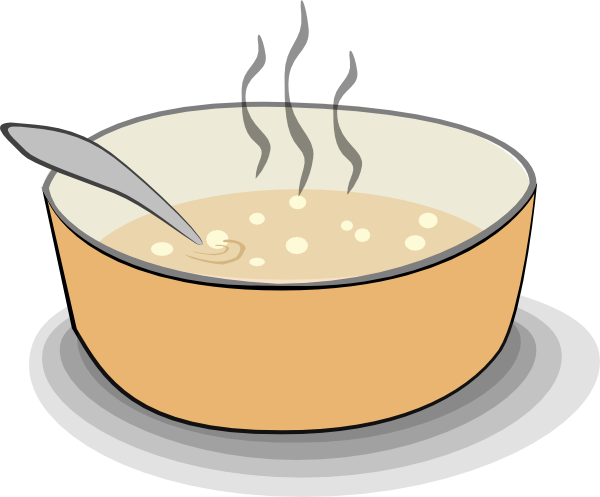
\includegraphics[width=0.3\textwidth]{figures/soup}
\end{center}

\begin{itemize}

\item When you taste a spoonful of soup and decide the spoonful you tasted isn't salty 
enough, that's \alert{exploratory analysis}

\item If you generalize and conclude that your entire soup needs salt, that's an \alert{
inference}

\item For your inference to be valid, the spoonful you tasted (the sample) needs to be 
\alert{representative} of the entire pot (the population)

\end{itemize}
\end{frame}

%%%%%%%%%%%%%%%%%%%%%%%%%%%%%%%%%%%

\begin{frame}
\frametitle{Sampling is natural}
\begin{center}
\includegraphics<1>[width=0.5\textwidth]{figures/tacobowl.jpg}
\includegraphics<2>[width=1\textwidth]{figures/tacobowl_close.jpg}
\end{center}
\end{frame}
%%%%%%%%%%%%%%%%%%%%%%%%%%%%%%%%%%%

\section{Ideally use a simple random sample, stratify to control for a variable, and cluster to make sampling easier} 
\label{mi2}

%%%%%%%%%%%%%%%%%%%%%%%%%%%%%%%%%%%
\begin{frame}


\twocol{0.505}{0.51}{
\alert{Simple random:} \\
{\small Drawing names from a hat}
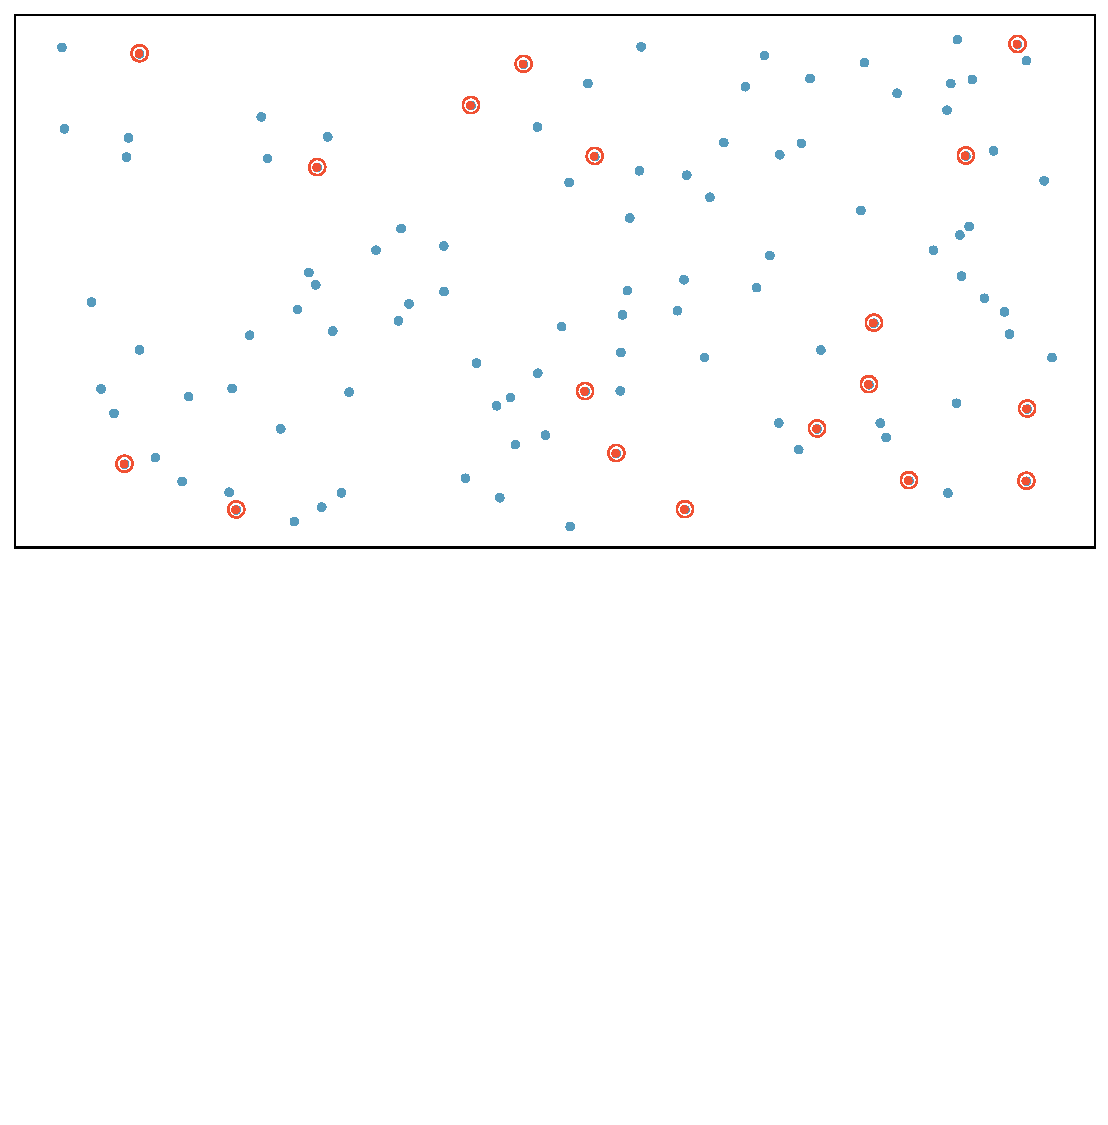
\includegraphics[width=\textwidth]{figures/sampling_simple} \\
\pause
\alert{Stratified:} {\small homogenous strata} \\
{\small Stratify to control for SES} \\
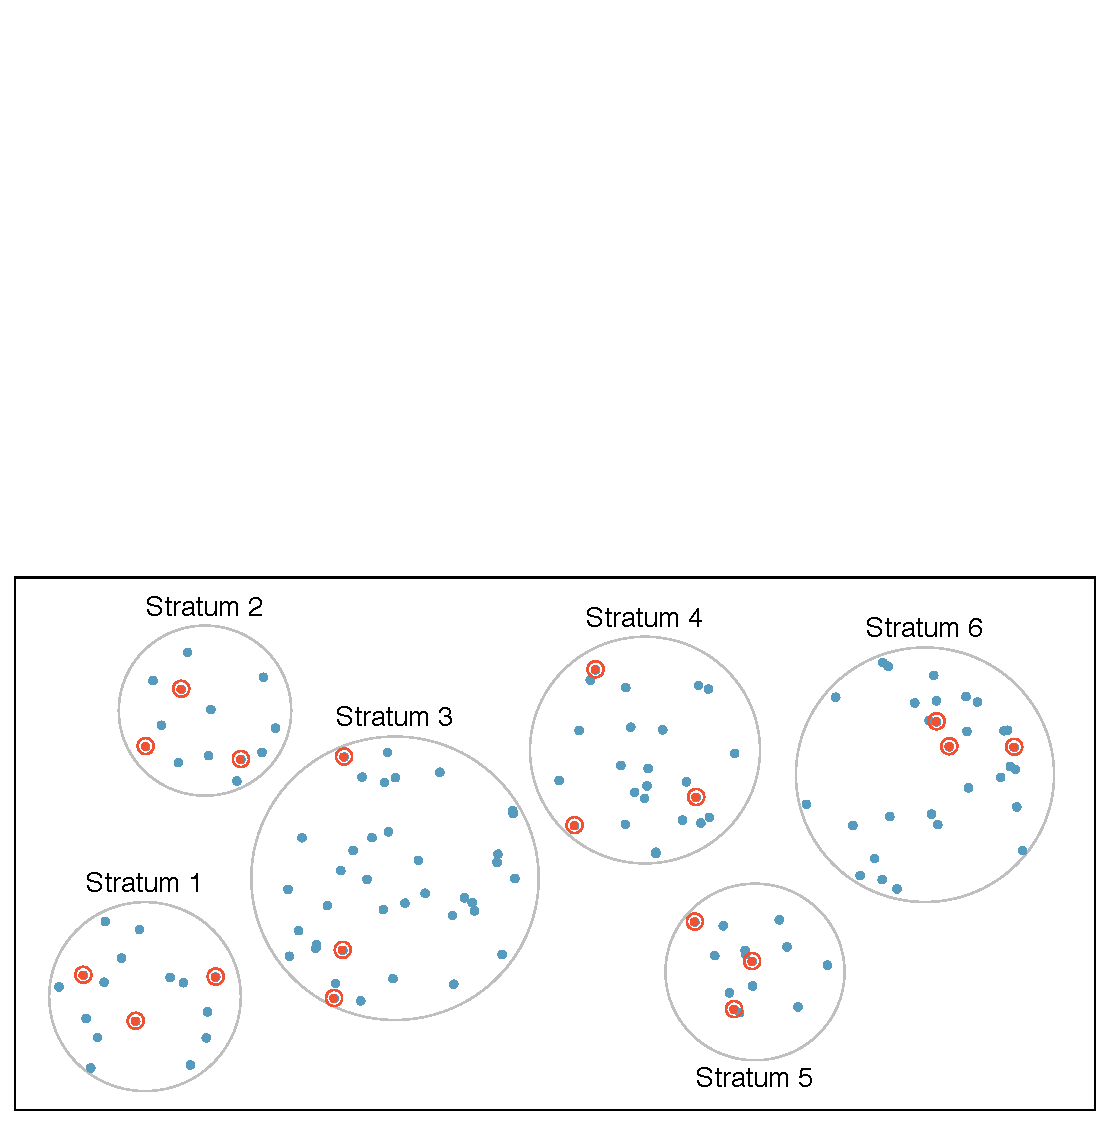
\includegraphics[width=\textwidth]{figures/sampling_stratified} 
}
{
\pause
\alert{Cluster:} {\small heterogenous clusters} \\
{\small Sample all chosen clusters}
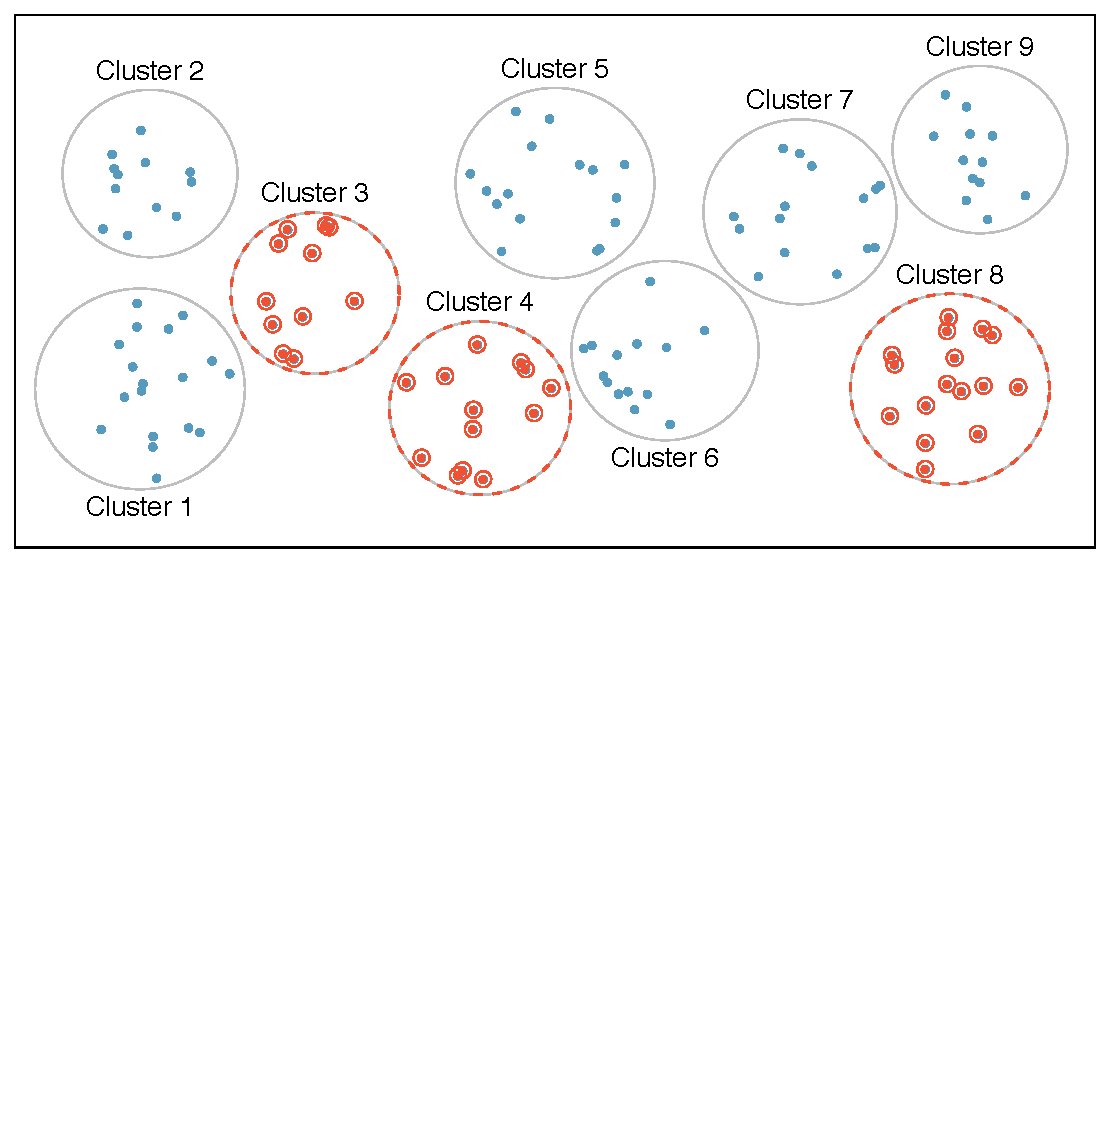
\includegraphics[width=\textwidth]{figures/sampling_cluster} \\
\pause
\alert{Multistage:} \\
{\small Random sample in chosen clusters}
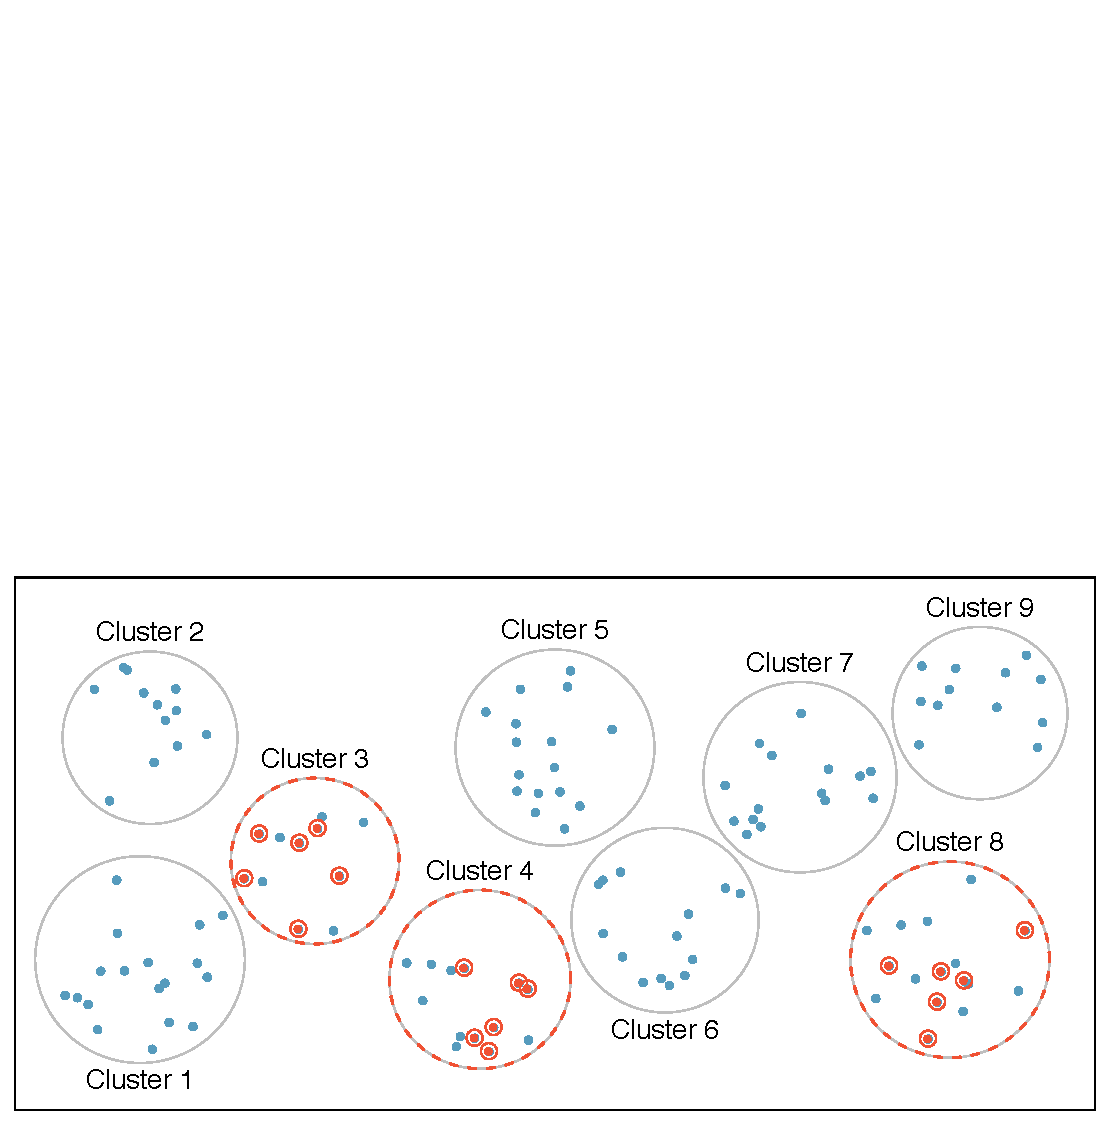
\includegraphics[width=\textwidth]{figures/sampling_multistage}
}

\end{frame}

%%%%%%%%%%%%%%%%%%%%%%%%%%%%%%%%%%%

\begin{frame}
\footnotesize{
\begin{exampleblock}{Your Turn}
A city council has requested a household survey be conducted in a suburban 
area of their city. The area is broken into many distinct and unique neighborhoods, 
some including large homes, some with only apartments, and others a diverse mixture of 
housing structures. Which approach would likely be the \emph{least} effective?\end{exampleblock}}

\begin{enumerate}[(a)]
\item Simple random sampling
\item Stratified sampling, where each stratum is a neighborhood
\item \textitMult{Cluster sampling, where each cluster is a neighborhood}
\end{enumerate}

\end{frame}

%%%%%%%%%%%%%%%%%%%%%%%%%%%%%%%%%%%

\section{Sampling schemes can suffer from a variety of biases}
\label{mi3}

%%%%%%%%%%%%%%%%%%%%%%%%%%%%%%%%%%%

\begin{frame}
\frametitle{3. Sampling schemes can suffer from a variety of biases}

\begin{itemize}[<+->]

\item \alert{Non-response:} If only a small fraction of the randomly sampled people choose 
to respond to a survey, the sample may no longer be representative of the population

\item \alert{Voluntary response:} Occurs when the sample consists of people who volunteer 
to respond because they have strong opinions on the issue since such a sample will also 
not be representative of the population

\item \alert{Convenience sample:} Individuals who are easily accessible are more likely to 
be included in the sample

\end{itemize}

\end{frame}

%%%%%%%%%%%%%%%%%%%%%%%%%%%%%%%%%%%

\begin{frame}[shrink]

{\small
\footnotesize{
\begin{exampleblock}{Your Turn}
A school district is considering whether it will no longer allow high school 
students to park at school after two recent accidents where students were severely 
injured. As a first step, they survey parents by mail, asking them whether or not the 
parents would object to this policy change. Of 6,000 surveys that go out, 1,200 are 
returned. Of these 1,200 surveys that were completed, 960 agreed with the policy change 
and 240 disagreed. Which of the following statements are true?
\end{exampleblock}}

\begin{enumerate}[I.]
\item Some of the mailings may have never reached the parents.
\item Overall, the school district has strong support from parents to move forward with 
the policy approval.
\item It is possible that majority of the parents of high school students disagree with 
the policy change.
\item The survey results are unlikely to be biased because all parents were mailed a 
survey. 
\end{enumerate}

\begin{multicols}{5}
\begin{enumerate}[(a)]
\item Only I
\item I and II
\item \textitMult{I and III}
\item III and IV
\item Only IV
\end{enumerate}
\end{multicols}
}

\end{frame}

%%%%%%%%%%%%%%%%%%%%%%%%%%%%%%%%%%%%

\section{Experiments use random assignment to treatment groups, observational studies do not}
\label{mi4}

%%%%%%%%%%%%%%%%%%%%%%%%%%%%%%%%%%%%

\begin{frame}

\begin{exampleblock}{}
What type of study is this? What is the scope of inference (causality / generalizability)?\footnote{http://www.nytimes.com/2014/06/30/technology/facebook-tinkers-with-users-emotions-in-news-feed-experiment-stirring-outcry.html}
\end{exampleblock}
\begin{center}
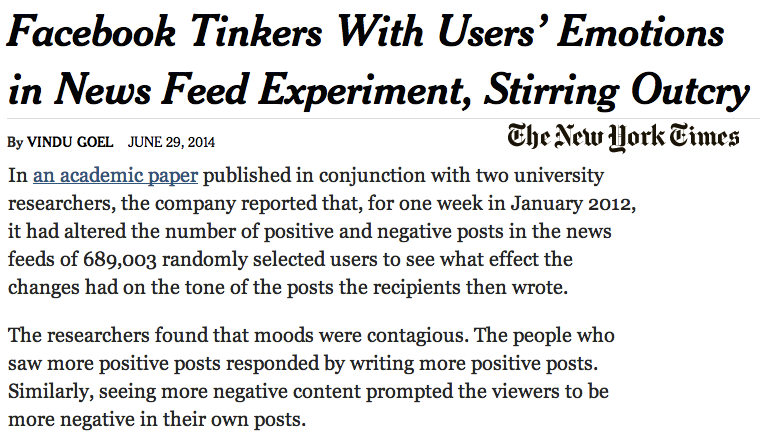
\includegraphics[width=0.9\textwidth]{figures/facebook_study}
\end{center}
%\scriptsize{
%\alert{\url{http://www.nytimes.com/2014/06/30/technology/facebook-tinkers-with-users-emotions-in-news-feed-experiment-stirring-outcry.html}}}

\end{frame}

%%%%%%%%%%%%%%%%%%%%%%%%%%%%%%%%%%%%%

\begin{frame}
\frametitle{4. Experiments use random assignment to treatment groups, observational studies do not}

{\small
\begin{exampleblock}{Your Turn}A study that surveyed a random sample of otherwise healthy adults found that people are more likely to get muscle cramps when they're stressed. The study also noted that people drink more coffee and sleep less when they're stressed. What type of study is this?
\end{exampleblock}

\textit{\onslide<2->{Observational}}

\begin{exampleblock}{What is the conclusion of the study?}\end{exampleblock}

\textit{\onslide<3->{There is an \alert{association} between increased stress \& muscle cramps.}}

\begin{exampleblock}{Can this study be used to conclude a causal relationship between increased stress and muscle cramps?}\end{exampleblock}

\textit{\onslide<4->{Muscle cramps might also be due to increased caffeine consumption or sleeping less -- these are potential \alert{confounding} variables.}}
}

\end{frame}

%%%%%%%%%%%%%%%%%%%%%%%%%%%%%%%%%%%%

\section{Four principles of experimental design: randomize, control, block, replicate}
\label{mi5}

%%%%%%%%%%%%%%%%%%%%%%%%%%%%%%%%%%%%

\begin{frame}
\frametitle{5. Four principles of experimental design:\\ randomize, control, block, 
replicate}

\begin{itemize}
\item We would like to design an experiment to investigate if increased stress causes 
muscle cramps:

\pause

\begin{itemize}
\item Treatment: increased stress
\item Control: no or baseline stress
\end{itemize}

\pause

\item It is suspected that the effect of stress might be different on younger and older 
people: \alert{block} for age.

\end{itemize}

\pause

\begin{alertblock}{Why is this important? Can you think of other variables to block for?}\end{alertblock}

\end{frame}

%%%%%%%%%%%%%%%%%%%%%%%%%%%%%%%%%%%

\section{Random sampling helps generalizability, random assignment helps causality}
\label{mi6}

%%%%%%%%%%%%%%%%%%%%%%%%%%%%%%%%%%%%

\begin{frame}
\frametitle{6. Random sampling helps generalizability,\\ random assignment helps 
causality}

\begin{center}
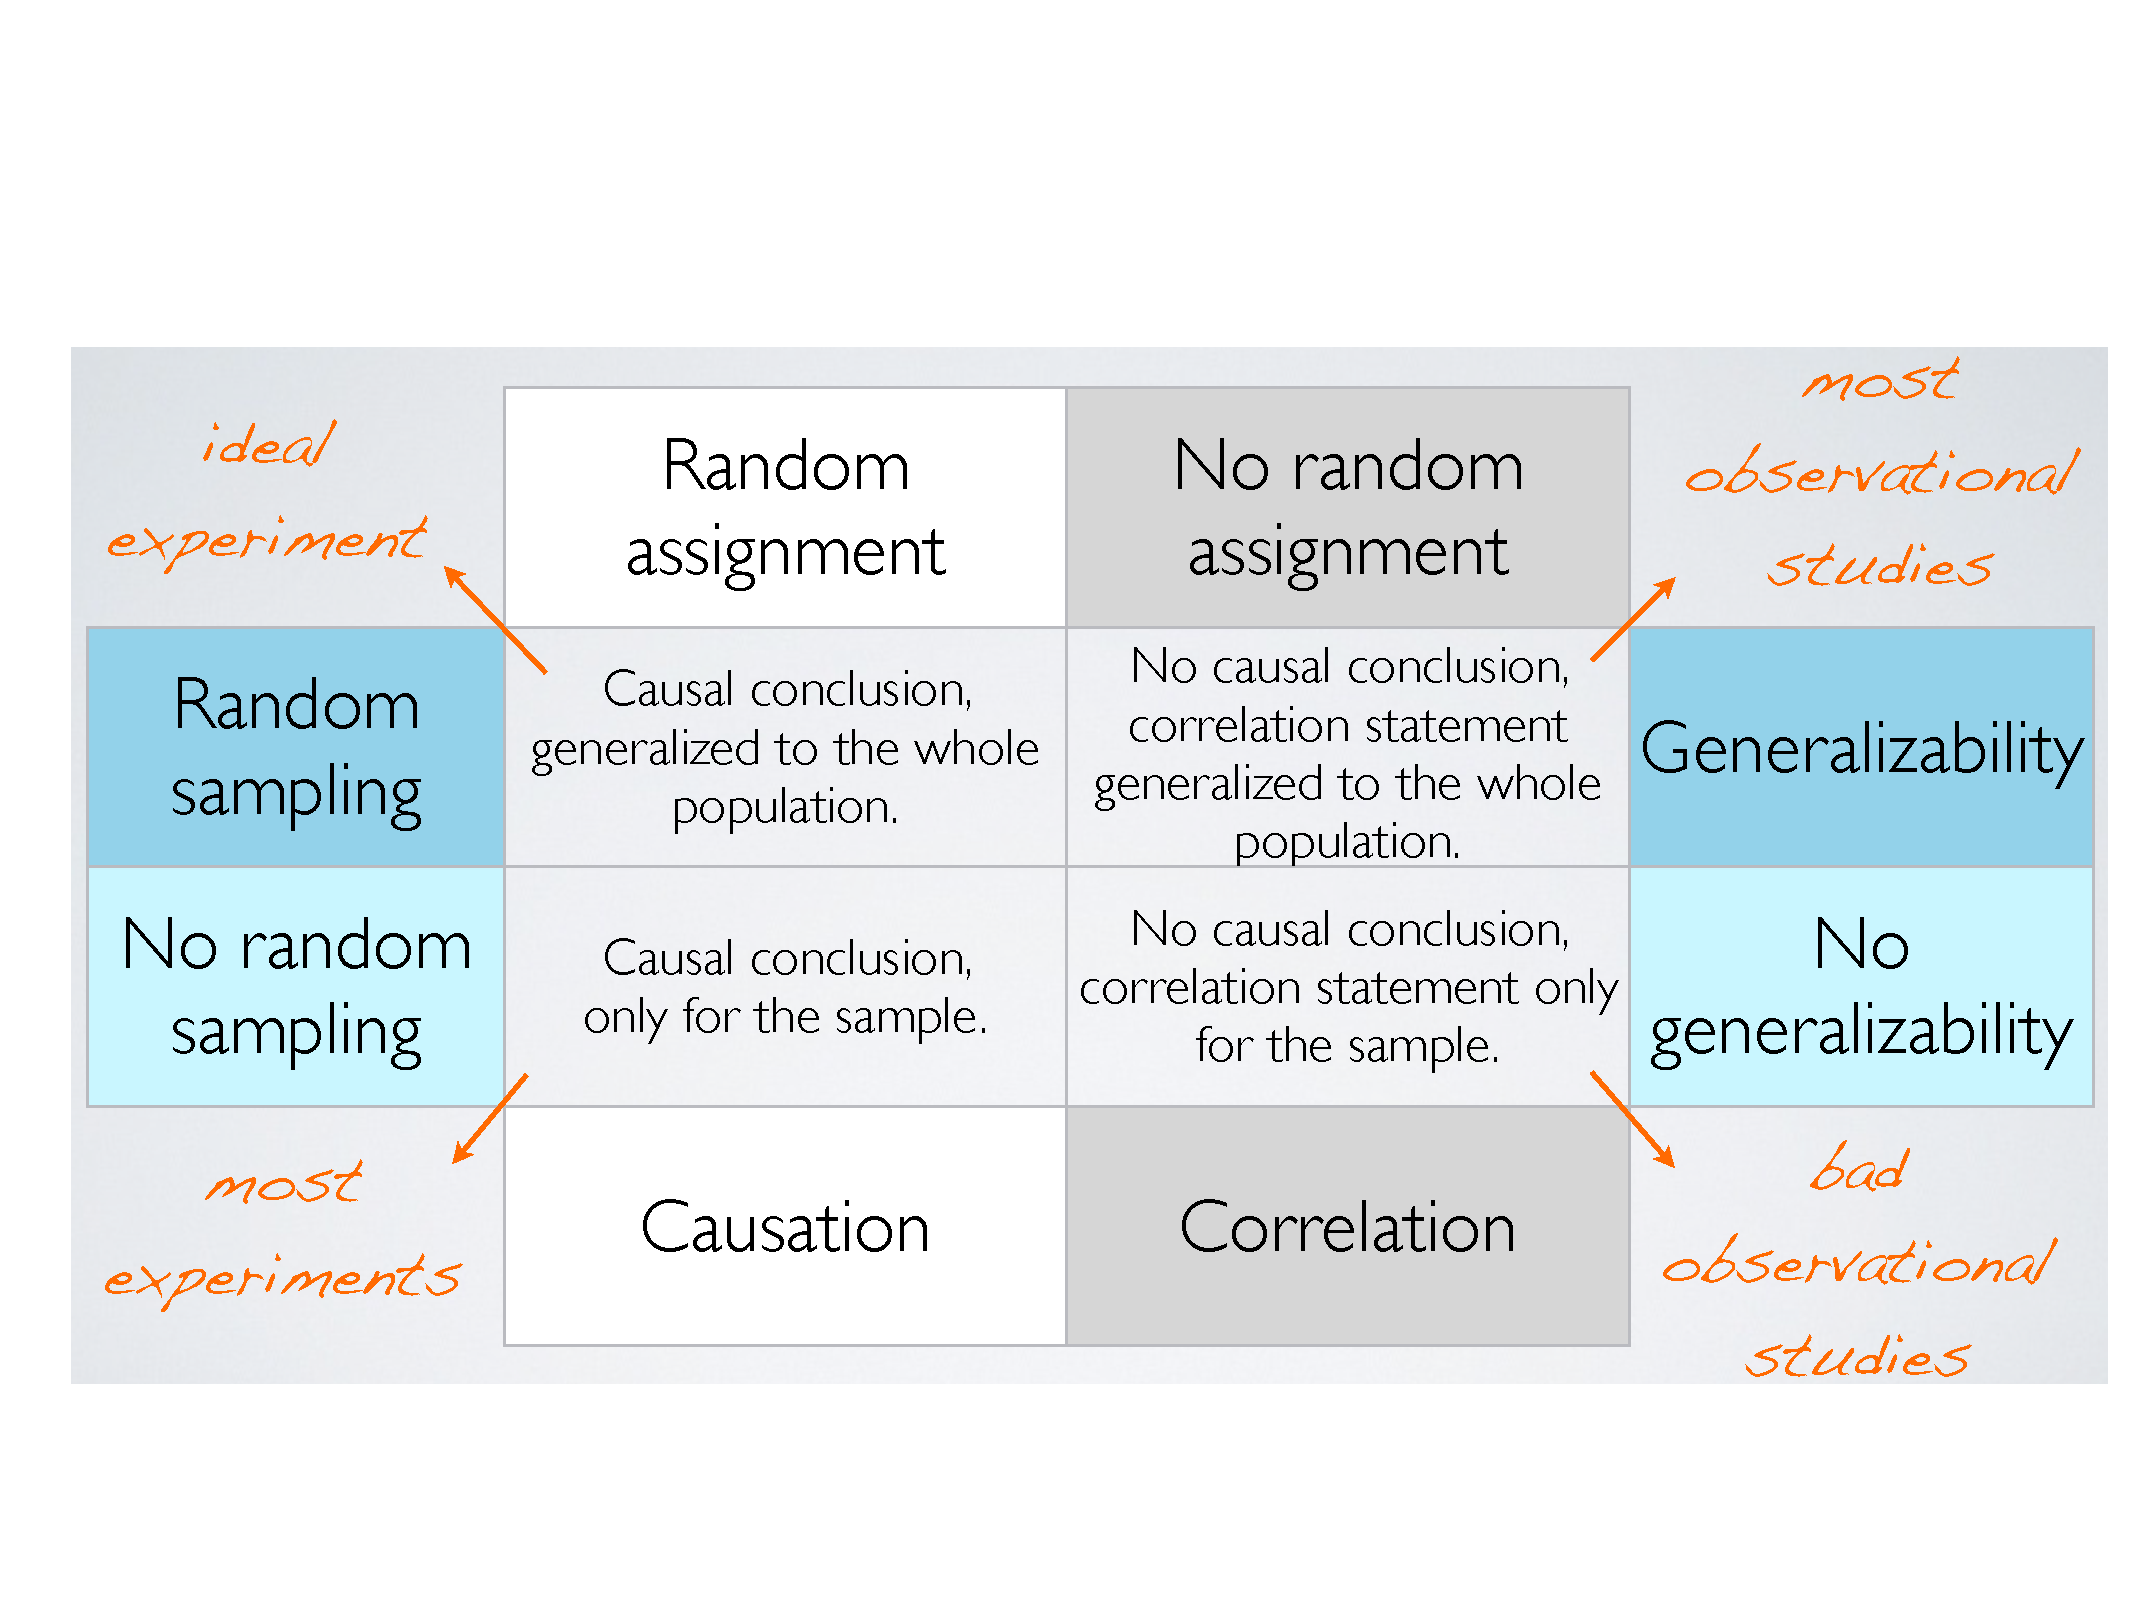
\includegraphics[width=\textwidth]{figures/random_sample_assignment}
\end{center}

\end{frame}

%%%%%%%%%%%%%%%%%%%%%%%%%%%%%%%%%%%

\section{Summary}

%%%%%%%%%%%%%%%%%%%%%%%%%%%%%%%%%%%

\begin{frame}
\frametitle{Summary of main ideas}

\vfill

\begin{enumerate}

\item \nameref{mi1}

\item \nameref{mi2}

\item \nameref{mi3}

\item \nameref{mi4}

\item \nameref{mi5}

\item \nameref{mi6}

\end{enumerate}

\vfill

\end{frame}
%%%%%%%%%%%%%%%%%%%%%%%%%%%%%%%%%%%

%%%%%%%%%%%%%%%%%%%%%%%%%%%%%%%%%%%
%%%%%%%%%%%%%%%%%%%%%%%%%%%%%%%%%%%
\begin{frame}[standout]
\Large{Exploratory data analysis}
\end{frame}
%%%%%%%%%%%%%%%%%%%%%%%%%%%%%%%%%%%
%%%%%%%%%%%%%%%%%%%%%%%%%%%%%%%%%%%


\section{Always start your exploration with a visualization}
\label{mi7}

%%%%%%%%%%%%%%%%%%%%%%%%%%%%%%%%%%%

\begin{frame}[fragile]
\frametitle{From a class survey...}

\alert{Do you see anything out of the ordinary?}

\begin{center}
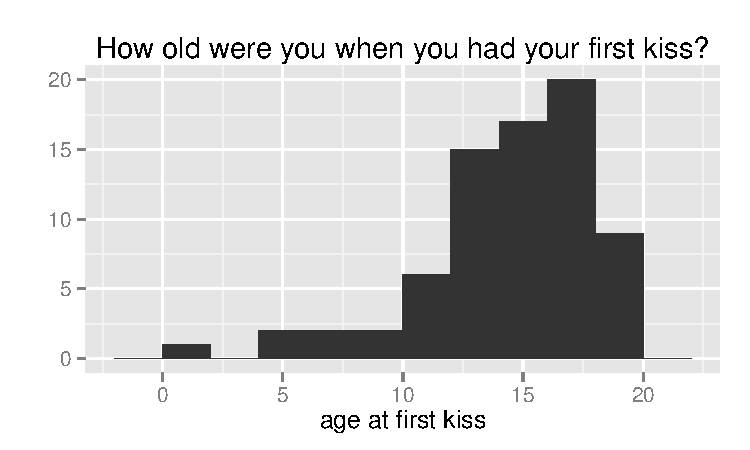
\includegraphics[width=0.8\textwidth]{figures/survey/hist_first_kiss} 
\end{center}

\pause

\soln{Some people reported very low ages, which might suggest the survey
  question wasn't clear: romantic kiss or any kiss?}

%---Note---%
\note{

To day we are going to talk about exploratory data analysis.

- the important thing is to always start your exploratory data analysis with
visualization.

- is there anything out of the ordinary about this?  you probably were first
kissed when you were a baby, but it isn't clear what we are talking about.

- so this is an example of how we need to be careful how we phrase a question.
we want to phrase it so that there is only one interpretation.

}

\end{frame}

%%%%%%%%%%%%%%%%%%%%%%%%%%%%%%%%%%%

\begin{frame}[fragile]
\frametitle{From a class survey...}

\alert{How are people reporting lower vs. higher values of FB visits?}

\begin{center}
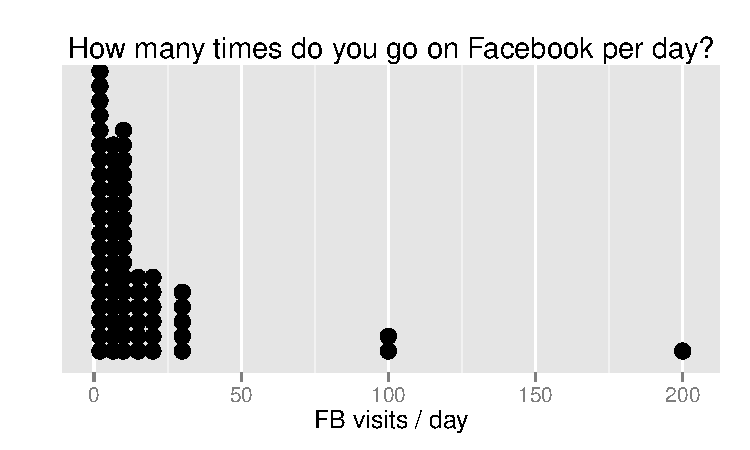
\includegraphics[width=0.8\textwidth]{figures/survey/dot_fb_visits_per_day} 
\end{center}

\pause

\soln{Finer scale for lower numbers.}

%---Note---%
\note{

How many people reporting lower vs. higher values of FB?  It is either 100 or
200, not 107, 113.

We can see that if you don't give guidance on data then it can be tough to
analyze.

}

\end{frame}

%%%%%%%%%%%%%%%%%%%%%%%%%%%%%%%%%%%

\begin{frame}
\frametitle{}

\alert{Describe the spatial distribution of preferred sweetened carbonated beverage drink.}

\begin{center}
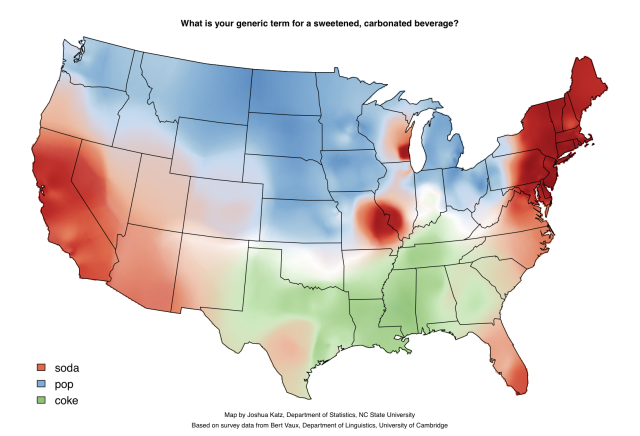
\includegraphics[width=0.9\textwidth]{figures/spatial/soda}
\end{center}


%---Note---%
\note{

How do we refer to these maps?

An intensity map.

Do people call their sweetened carbontated drink pop, etc.

Describe how people do.

Really we are looking at two variables: geographic location and terminology.

}

\end{frame}

%%%%%%%%%%%%%%%%%%%%%%%%%%%%%%%%%%%

\begin{frame}
\frametitle{}

\alert{What is missing in this visualization?}

\begin{center}
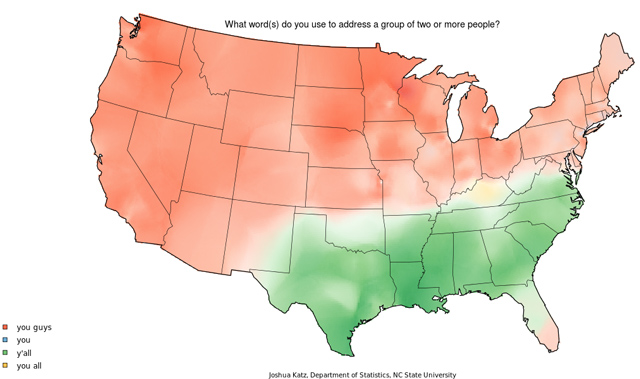
\includegraphics[width=0.9\textwidth]{figures/spatial/yalls}
\end{center}


%---Note---%
\note{

 How do you address a group.

 Describe.

 What do you think is missing in this visualization.

 What would be useful beyond the colors?  What does the shade of the color
 represent?  We have no idea of what value it corresponds to?

 It is missing some information about the numerical intensity that would help us
 compare across colors

 Important point: always start with a visualization.

}

\end{frame}

%%%%%%%%%%%%%%%%%%%%%%%%%%%%%%%%%%

\section{When describing numerical distributions discuss shape, center, spread, and unusual observations}
\label{mi8}

%%%%%%%%%%%%%%%%%%%%%%%%%%%%%%%%%%%

\begin{frame}
\frametitle{Describing distributions of numerical variables}

\begin{itemize}

\item \alert{Shape}: skewness, modality

\item \alert{Center}: an estimate of a \alert{typical} observation in the distribution (mean, median, mode, etc.) 
\begin{itemize}
\item Notation: $\mu$: population mean, $\bar{x}$: sample mean
\end{itemize}

\item \alert{Spread}: measure of variability in the distribution (standard deviation, IQR, range, etc.)

\item \alert{Unusual observations}: observations that stand out from the rest of the data that may be suspected outliers

\end{itemize}

%---Note---%
\note{

  Always talk about shape, center, spread, etc.

  Shape

  What do I mean by modality: promenent peaks.

  When talking about center, what is most common measure of center: mean

  What else: median.

  Mode is also used, though it isn't always that useful.  It is the most
  frequent observation.  But it is sometimes hard to determine what that is when
  working with continuous numerical data.

  Just a note for notation: $\mu$ or any greek letter denotes a pop. param.
  $\mu$ is pop bar.

  xbar is a sample statistic.  Often times we want to know mu, but we don't have
  pop, so we caompute xbar and call that best guess.

  how can we put some uncertainty around best guess to refelect that this comes
  from sample and not whole pop.

  when we talk about spread we are talking about variability in the distribution.

  unusual observations.  sometimes people just remove outliers.  you should not
  do that unless you have good reason to do so, they may convey important information.

}

\end{frame}

%%%%%%%%%%%%%%%%%%%%%%%%%%%%%%%%%%

\begin{frame}
\frametitle{}

\begin{exampleblock}{Your Turn}Which of these is most likely to have a roughly symmetric distribution?\end{exampleblock}
\begin{enumerate}[(a)]
\item salaries of a random sample of people from NY
\item \solnMult{weights of adult females}
\item scores on an well-designed exam
\item last digits of phone numbers
\end{enumerate}

%---Note---%
\note{

which of the following is mostly likely to have a roughly symmetric
distribution.

things all over the place.  talk to each other and vote again.

let them have a minute.  Make sure to go again whether you changed your answer
or not.

C is now most popular.

if i were to design example that was symmetic, you would be in trouble.  what is
max, what is min.  so what would this look like.  can everyone get 90s and
above.

usually scores on a well designed exam are left skewed.  decent center, but not
at 100.

left or right skewed?

left.

what about b?  some aveerage weight.  Do we expect sampe number to be above and
below?  we don't expect one end to be more frequent than others.

what about random samples of salary from nc.  what we we expect the shape of
that to be?

last digits of phone numbers?  what type of shape might we expect?  there is not
one digit that is more popular than the others.n

}

\end{frame}

%%%%%%%%%%%%%%%%%%%%%%%%%%%%%%%%%%%

\begin{frame}
\frametitle{Mean vs. median}

\begin{exampleblock}{Your Turn} How do the mean and median of the following two datasets compare? \\
$\:$\\
Dataset 1: 30, 50, 70, 90 \\
Dataset 2: 30, 50, 70, 1000
\end{exampleblock}

\begin{enumerate}[(a)]
\item $\bar{x}_1 = \bar{x}_2$, $median_1 = median_2$
\item \solnMult{$\bar{x}_1 < \bar{x}_2$, $median_1 = median_2$}
\item $\bar{x}_1 < \bar{x}_2$, $median_1 < median_2$
\item $\bar{x}_1 > \bar{x}_2$, $median_1 < median_2$
\item $\bar{x}_1 > \bar{x}_2$, $median_1 = median_2$
\end{enumerate}

%---Note---%
\note{

how do the mean and median of the following compare.  do by yourself first.

give you a minute.

b is the winner.  everyone got it.

% can I explain this in words?

what is the idea we are getting at here?  some extreme value is affecting the
mean, but not the median.  so it is more robust.

}

\end{frame}

%%%%%%%%%%%%%%%%%%%%%%%%%%%%%%%%%%%

\begin{frame}
\frametitle{Standard deviation and variance}

\begin{itemize}

\item Most commonly used measure of variability is the \alert{standard deviation}, which roughly measures the average deviation from the mean
\begin{itemize}
\item Notation: $\sigma$: population standard deviation, $s$: sample standard deviation
\end{itemize}

\item Calculating the standard deviation, for a population (rarely, if ever) and for a sample:

\[ \darkgray{$\sigma = \sqrt{\frac{\sum_{i = 1}^N (x_i - \mu)^2}{n}}$} \qquad s = \sqrt{\frac{\sum_{i = 1}^n (x_i - \bar{x})^2}{n - 1}} \]


\item Square of the standard deviation is called the \alert{variance}.

\end{itemize}

%---Note---%
\note{

spread.  here we are going to go about standard deviation.

one of the more tedious computations.

it roughly measures the average deviation from the mean.

we want to think about how far or how close the data are from the mean on
average.

notation: sigma, greek population standard deviation.  s: sample standard
deviation.

gray here is population data, we rarely have this.

a couple things: used square.  and divide by $n-1$.

why use squares.

standard deviation is nice because it is the same units as what you measure.

}

\end{frame}

%%%%%%%%%%%%%%%%%%%%%%%%%%%%%%%%%%%

\begin{frame}
\frametitle{More on SD}

\alert{Why divide by $n - 1$ instead of $n$ when calculating the sample standard deviation?}

\pause

Lose a ``degree of freedom" for using an estimate (the sample mean, $\bar{x}$), in estimating the sample variance/standard deviation.

\pause

$\:$ \\

\alert{Why do we use the squared deviation in the calculation of variance?}

\pause

\begin{itemize}
\item To get rid of negatives so that observations equally distant from the mean are weighed equally.
\item To weigh larger deviations more heavily.
\end{itemize}

%---Note---%
\note{

why divide by $n-1$ instead of $n$?

go back.  compare equations.  ideally use population mean.  this introduces
extra uncertatiny.  for that we need to penalize ourselves.

if i divide by $n-1$ or $n$ which yields a higher value?  if i divide by
something smaller, I get a larger number.

so we are in effect reporting a larger estimate of the standard deviation.  this
is conservative.

go forward.  why square things?  what happens if we add a positive and a
negative number?  they cancel out.

one reasons, you don't want positives and negatives to cancel.

what would be a more intuitive way?

abs.

what does square do?  it weights larger deviations more heavily?

}

\end{frame}

%%%%%%%%%%%%%%%%%%%%%%%%%%%%%%%%%%%

\begin{frame}
\frametitle{Range and IQR}

\begin{exampleblock}{Our Turn}For the given data set: 7, 6, 5, 5, 9, 10, 11, 10, 9 \\
Calculate 
\begin{itemize}
\item Range
\item Median
\item The three quartiles 
\item Interquartile range (IQR)
\item Draw a boxplot 
\end{itemize}
\end{exampleblock}




%---Note---%
\note{

Give about 45 seconds.

many yeses some nos.  can i hear from someone that said no?

what is definition of iqr.

what is definition of range.

is the range or iqr more robust to iqr robust to outliers?  outliers are most
likely minimum or maximum points.  calculation of range is based on exactly
these values.


}

\end{frame}

%%%%%%%%%%%%%%%%%%%%%%%%%%%%%%%%%%%

\section{Robust statistics are not easily affected by outliers and extreme skew}
\label{mi9}

%%%%%%%%%%%%%%%%%%%%%%%%%%%%%%%%%%%

\begin{frame}
\frametitle{Robust statistics}

\begin{itemize}

\item Mean and standard deviation are easily affected by extreme observations since the value of each data point contributes to their calculation.

\item Median and IQR are more robust.

\item Therefore we choose median\&IQR (over mean\&SD) when describing skewed distributions.

\end{itemize}

%---Note---%
\note{

median and iqr are robust.  this is why use them do describe skewed
distribution.

which is more informative for skewed distribution?

when describing dist, first think about shape, then think about numbers to use
to describe.

it is on you to get an idea on visualization and then pick.


}

\end{frame}

%%%%%%%%%%%%%%%%%%%%%%%%%%%%%%%%%%%

\section{Use box plots to display quartiles, median, and outliers}
\label{mi10}

%%%%%%%%%%%%%%%%%%%%%%%%%%%%%%%%%%%

\begin{frame}
\frametitle{Box plot}

A \alert{box plot} visualizes the median, the quartiles, and suspected outliers. An \alert{outlier} is defined as an observation more than 1.5$\times$IQR away from the quartiles.

\begin{center}
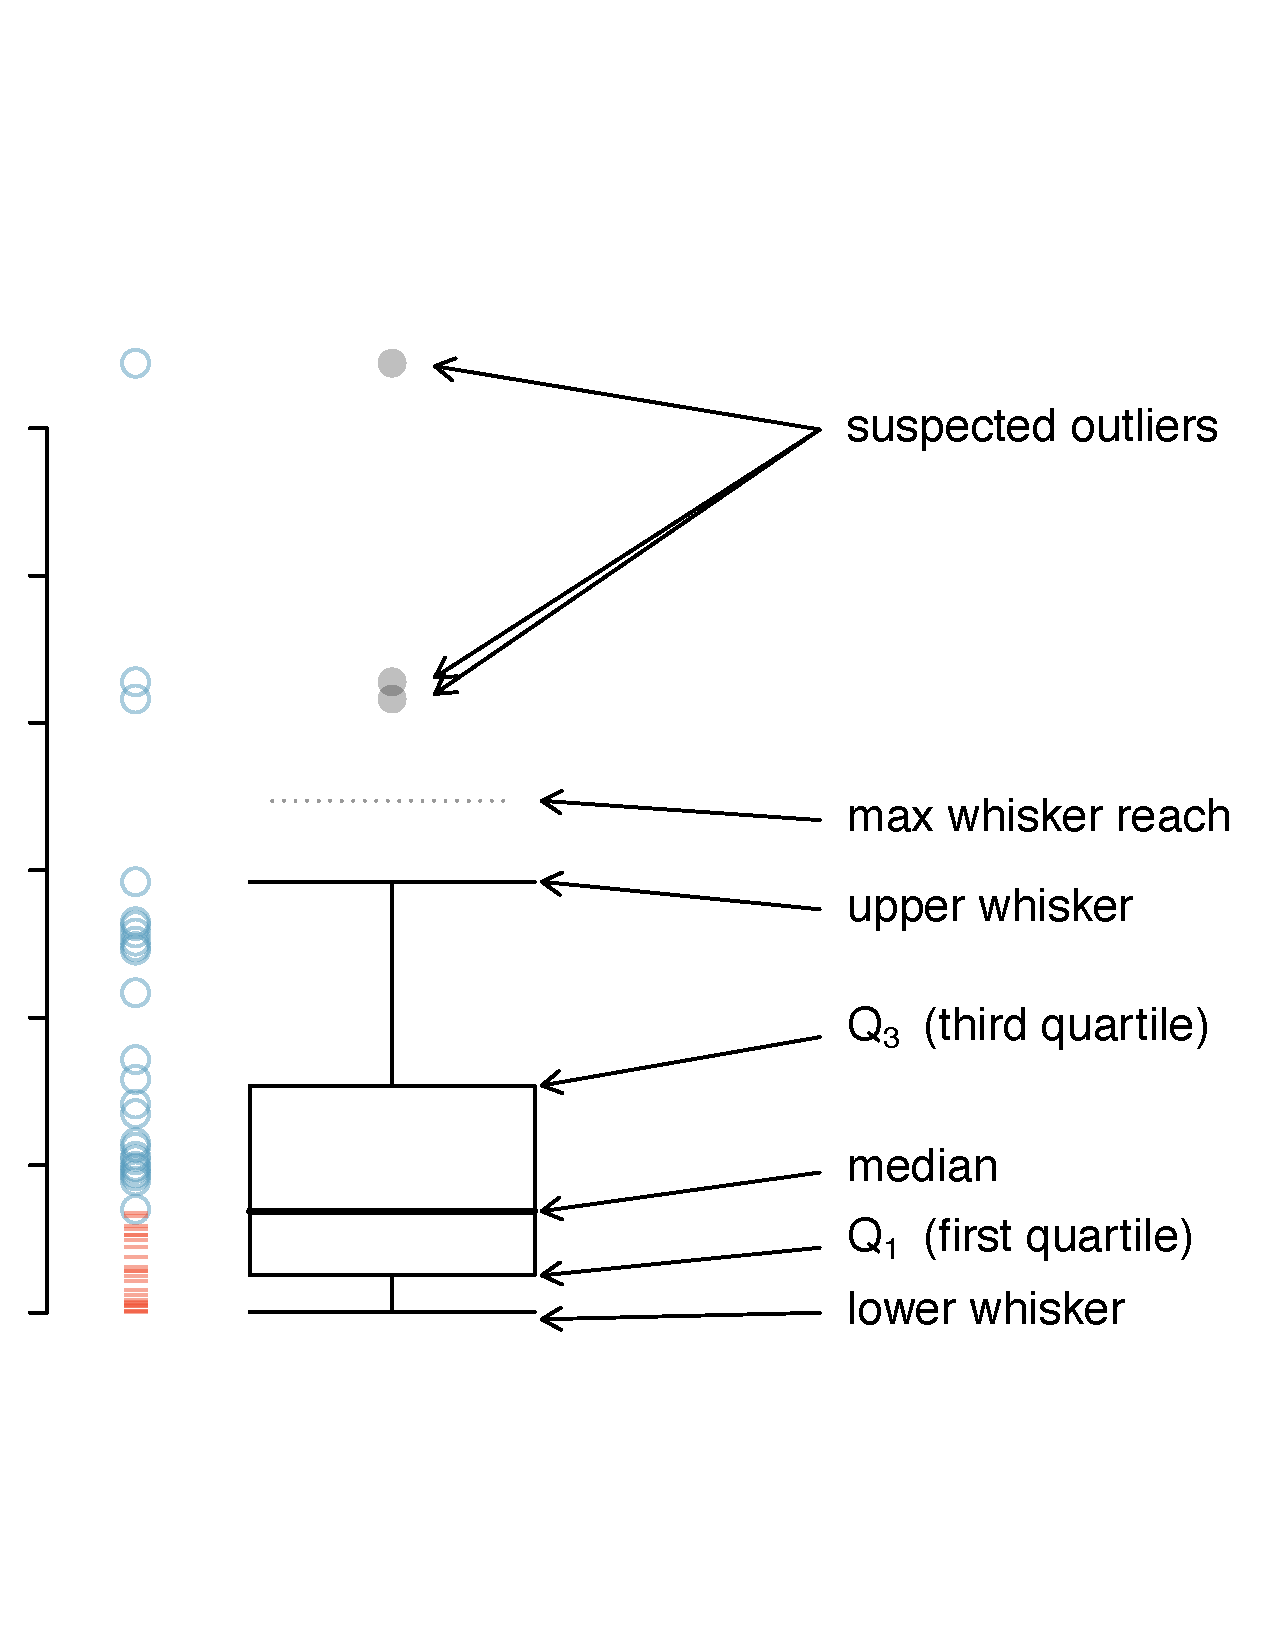
\includegraphics[width=0.6\textwidth]{figures/boxPlotLayoutNumVar}
\end{center}

%---Note---%
\note{

boxplot is useful for median, iqr.

data set of 5, where will the median be.

if 6, where will it be?

boxplots are good for showing where outliers are.

fence: 1.5 iqr.

explain whiskers.  whiskers are 1.5 from interquartile range.

}

\end{frame}

%%%%%%%%%%%%%%%%%%%%%%%%%%%%%%%%%%%


\begin{frame}
\frametitle{}

\vfill

\begin{alertblock}{Aplication Exercise}{1.1 Distributions of numerical variables}\end{alertblock}
\vfill

%---Note---%
\note{

you get 10 minutes to work on in teams.

randomly pick a team to discuss answers on board.

make sure you are concise, but clear.

1. 

a: digits
b: marriage

2. 

a: 2
b: 1 why 1 and not 4?
c: 6: right skewed
d: 3: a few people pulling all nighters
e: 4: on campus
f: 5: what do we think the numbers are?  what are most common?

3. think about numerical/categorical (are we looking at bar plot or histogram);
think about natural boundaries---there is a lower bound on piercings; then think
about shape: skew, symmetry, think about the modes.

4. Need to actually compute.

team claimed, a, c, b for variability.

Be careful about explain your reasoning.

5. E is more variable. 

Be careful about explain your reasoning.  more values that are closer to the
mean.

variability vs diversity.  diversity is not smooth.

Ask if people need more time.  Tell people they are welcome to go onto next app
ex if they are done.

Make sure you go ahead and submit your responses.

state names.

}

\end{frame}

%%%%%%%%%%%%%%%%%%%%%%%%%%%%%%%%%%%%

\section{Summary}

%%%%%%%%%%%%%%%%%%%%%%%%%%%%%%%%%%%%

\begin{frame}
\frametitle{Summary of main ideas}

\vfill

\begin{enumerate}

\item \nameref{mi7}

\item \nameref{mi8}

\item \nameref{mi9}

\item \nameref{mi10}

\end{enumerate}

\vfill

\end{frame}

%%%%%%%%%%%%%%%%%%%%%%%%%%%%%%%%%%%

\section{Polling and the Public}

\begin{frame}{The Importance of Public Opinion Polling}

\begin{itemize}

\item Do you think public opinion polls are an accurate reflection of what people actually think? Why or why not? \pause
\item How can public opinion polls influence policy decisions? Can this be a positive or negative thing? \pause
\item What are some of the challenges of measuring public opinion? \pause
\item How can citizens become more informed consumers of public opinion polls? \pause
\item Do you think public opinion polls can be harmful to democracy? If so, how?

\end{itemize}

\end{frame}


\begin{frame}{The Nuts and Bolts of Polling}
\begin{itemize}
\item What are the different types of sampling methods used in public opinion polls? How do they affect the accuracy of the results? \pause
\item How can the wording of a question influence the response of a pollster? \pause
\item What are some of the ethical considerations involved in conducting public opinion polls? \pause
\item How can citizens determine whether a poll is reliable and trustworthy? \pause
\item What are some of the limitations of using public opinion polls to make predictions about elections or other events?
\end{itemize}
\end{frame}



\section{Sample surveys in our electronic world}




\begin{frame}{The Diversity of Surveys}

Surveys are conducted for a great variety of reasons within all sorts of populations
They can vary in size, scope, and how they are administered

But surveys are all motivated by the desire to collect information that can answer a particular question or solve a specific problem
\end{frame}

\begin{frame}{The Power of Sample Surveys}
Census: a survey that includes every member of the target population

Sample survey: a survey that includes only some members of the target population

Surveys using probability-based samples allow one to make estimates about the target population by surveying only some members of that population 

Probability sample surveys are much more efficient than conducting a census—they can save time and resources
\end{frame}

\begin{frame}{Four Sources of Survey Error}
Survey error occurs when the estimate that is produced using survey data is different from the true value of the variable in the population one hopes to describe
There are four main types of error that surveyors must attempt to minimize
No source of error can be ignored
\end{frame}

\begin{frame}{1. Coverage Error}
Occurs when the list of members of the target population from which sample members are drawn (the sample frame) does not accurately reflect the population on the characteristic(s) the survey is trying to estimate
Coverage error is the difference between the estimate produced when the list is inaccurate and what would have been produced with an accurate list
A high-quality sample survey requires that every member of the population has a known, nonzero probability of being sampled. If some units are not on the list, there will be undercoverage
\end{frame}

\begin{frame}{2. Sampling Error}
The difference between the estimate produced when only a sample of units is surveyed and the estimate produced when all units are surveyed
Occurs any time a survey includes only some, rather than all, members of the sampling frame; it is unavoidable in sample surveys
But it can be minimized, and probability sampling allows us to obtain estimates about the population within acceptable levels of precision by surveying only a small portion of the population
\end{frame}

\begin{frame}{3. Nonresponse Error}
The difference between the estimate produced when only some of the sampled units respond to the survey compared to when all of them respond
It occurs if those who don’t respond are different from those who do in a way that influences the estimate 
A high response rate can reduce the likelihood of nonresponse error, but it does not necessarily mean that there is low nonresponse error
\end{frame}

\begin{frame}{4. Measurement Error}
The difference between the estimate produced and the true value because respondents gave inaccurate answers
Respondents may be unwilling or unable to provide accurate answers for a variety of reasons: poor question design, survey mode effects, interviewer and respondent behavior, or data collection mistakes 
In some instances, measurement error is a result of specification error, which is when a question does not measure the concept it is intended to measure.
Yet, even if the question is a good way to measure a specific concept, there are many other ways in which measurement error can still occur

\end{frame}

\end{document}



\section{Sample surveys in our electronic world}




\begin{frame}{The Diversity of Surveys}



Surveys are conducted for a great variety of reasons within all sorts of populations
They can vary in size, scope, and how they are administered
But surveys are all motivated by the desire to collect information that can answer a particular question or solve a specific problem


\begin{frame}{The Power of Sample Surveys}
Census: a survey that includes every member of the target population
Sample survey: a survey that includes only some members of the target population
Surveys using probability-based samples allow one to make estimates about the target population by surveying only some members of that population 
Probability sample surveys are much more efficient than conducting a census—they can save time and resources


\begin{frame}{Four Sources of Survey Error}
Survey error occurs when the estimate that is produced using survey data is different from the true value of the variable in the population one hopes to describe
There are four main types of error that surveyors must attempt to minimize
No source of error can be ignored


\begin{frame}{1. Coverage Error}
Occurs when the list of members of the target population from which sample members are drawn (the sample frame) does not accurately reflect the population on the characteristic(s) the survey is trying to estimate
Coverage error is the difference between the estimate produced when the list is inaccurate and what would have been produced with an accurate list
A high-quality sample survey requires that every member of the population has a known, nonzero probability of being sampled. If some units are not on the list, there will be undercoverage
\begin{frame}{2. Sampling Error}
The difference between the estimate produced when only a sample of units is surveyed and the estimate produced when all units are surveyed
Occurs any time a survey includes only some, rather than all, members of the sampling frame; it is unavoidable in sample surveys
But it can be minimized, and probability sampling allows us to obtain estimates about the population within acceptable levels of precision by surveying only a small portion of the population

\begin{frame}{3. Nonresponse Error}
The difference between the estimate produced when only some of the sampled units respond to the survey compared to when all of them respond
It occurs if those who don’t respond are different from those who do in a way that influences the estimate 
A high response rate can reduce the likelihood of nonresponse error, but it does not necessarily mean that there is low nonresponse error


\begin{frame}{4. Measurement Error}
The difference between the estimate produced and the true value because respondents gave inaccurate answers
Respondents may be unwilling or unable to provide accurate answers for a variety of reasons: poor question design, survey mode effects, interviewer and respondent behavior, or data collection mistakes 
In some instances, measurement error is a result of specification error, which is when a question does not measure the concept it is intended to measure.
Yet, even if the question is a good way to measure a specific concept, there are many other ways in which measurement error can still occur

\begin{frame}{The Total Survey Error Framework}
Surveyors often make the mistake of attempting to reduce one particular source of error while ignoring others
Instead, surveyors should think in terms of minimizing total survey error (TSE)
This involves attempting to maximize data accuracy by simultaneously controlling all four sources of error to the extent practical and possible, within the time, cost, and other constraints of the survey


\begin{frame}{The Changing Survey Environment}
As technology continues to advance, there is an increasing number of ways to contact people and ask them to complete surveys
But, this also poses more obstacles to successful surveying
There is no longer a dominant survey mode, and single-mode surveys tend not to be as effective as they were in the past
Cultural norms have changed so that whether a person receives a survey request and responds rests more with the individual to whom the request is made, and not with the person making it


\begin{frame}{This Changing Environment Calls for a New Approach: Mixed-Mode Surveys}
This class emphasizes mixed-mode designs
This emphasis allows surveyors to keep the four sources of survey error at acceptably low levels and to reduce survey costs
But there are many other reasons why surveyors may use multiple modes
Mixing of modes may occur at the contact stage as well as the data collection stage

\begin{frame}{The Tailored Design Method (TDM)}
In order to minimize total survey error, surveyors must customize (tailor) their survey designs to fit their particular situations
There is no single set of design procedures that will work effectively in all situations
Surveyors must use knowledge of the survey topic, its sponsor, the types of people asked to participate, the resources available, and the time frame for reporting results to determine the best approach


\begin{frame}{Three Fundamental Considerations Underlie the TDM Approach}
A focus on reducing the four sources of error
Developing a set of procedures (including the recruitment contacts and the questionnaire) that interact and work together to encourage all sample members to respond
Developing survey procedures that build positive social exchange
A social exchange perspective suggests that people are more likely to respond to a questionnaire (and do so accurately) when they trust that the expected rewards for responding outweigh the expected costs




In your opinion, what are the most important things that citizens should know about public opinion polls?
How can we ensure that public opinion polls are used in a responsible and ethical way?
Do you think there are any situations where public opinion polls should not be conducted?